%%%%%%%%%%%%%%%%%%%%%%%%%%%%%%%%%%%%%%%%%
% Stylish Article
% LaTeX Template
% Version 2.1 (1/10/15)
%
% This template has been downloaded from:
% * <shivam.07@gmail.com> 2015-12-19T15:55:30.588Z:
%
% ^.
% http://www.LaTeXTemplates.com
%
% Original author:
% Mathias Legrand (legrand.mathias@gmail.com) 
% With extensive modifications by:
% Vel (vel@latextemplates.com)
%
% License:
% CC BY-NC-SA 3.0 (http://creativecommons.org/licenses/by-nc-sa/3.0/)
%
%%%%%%%%%%%%%%%%%%%%%%%%%%%%%%%%%%%%%%%%%

%----------------------------------------------------------------------------------------
%	PACKAGES AND OTHER DOCUMENT CONFIGURATIONS
%----------------------------------------------------------------------------------------

\documentclass[fleqn,12pt]{SelfArx} % Document font size and equations flushed left

\usepackage[english]{babel} % Specify a different language here - english by default
\usepackage{hyperref}
\usepackage{listings}
\usepackage{xcolor}
\newcommand{\quotes}[1]{``#1''}
%----------------------------------------------------------------------------------------
%	COLUMNS
%----------------------------------------------------------------------------------------

\setlength{\columnsep}{0.55cm} % Distance between the two columns of text
\setlength{\fboxrule}{0.75pt} % Width of the border around the abstract

%----------------------------------------------------------------------------------------
%	COLORS
%----------------------------------------------------------------------------------------

\definecolor{color1}{RGB}{0,0,90} % Color of the article title and sections
\definecolor{color2}{RGB}{0,20,20} % Color of the boxes behind the abstract and headings
\colorlet{punct}{red!60!black}
\definecolor{background}{HTML}{EEEEEE}
\definecolor{delim}{RGB}{20,105,176}
\colorlet{numb}{magenta!60!black}
\lstdefinelanguage{json}{
    basicstyle=\normalfont\ttfamily,
    numbers=left,
    numberstyle=\scriptsize,
    stepnumber=1,
    numbersep=8pt,
    showstringspaces=false,
    breaklines=true,
    frame=lines,
    backgroundcolor=\color{background},
    literate=
     *{0}{{{\color{numb}0}}}{1}
      {1}{{{\color{numb}1}}}{1}
      {2}{{{\color{numb}2}}}{1}
      {3}{{{\color{numb}3}}}{1}
      {4}{{{\color{numb}4}}}{1}
      {5}{{{\color{numb}5}}}{1}
      {6}{{{\color{numb}6}}}{1}
      {7}{{{\color{numb}7}}}{1}
      {8}{{{\color{numb}8}}}{1}
      {9}{{{\color{numb}9}}}{1}
      {:}{{{\color{punct}{:}}}}{1}
      {,}{{{\color{punct}{,}}}}{1}
      {\{}{{{\color{delim}{\{}}}}{1}
      {\}}{{{\color{delim}{\}}}}}{1}
      {[}{{{\color{delim}{[}}}}{1}
      {]}{{{\color{delim}{]}}}}{1},
}
\usepackage{listings}
\usepackage{color}

\definecolor{dkgreen}{rgb}{0,0.6,0}
\definecolor{gray}{rgb}{0.5,0.5,0.5}
\definecolor{mauve}{rgb}{0.58,0,0.82}

\lstset{frame=tb,
  language=Python,
  aboveskip=3mm,
  belowskip=3mm,
  showstringspaces=false,
  columns=flexible,
  basicstyle={\small\ttfamily},
  numbers=none,
  numberstyle=\tiny\color{gray},
  keywordstyle=\color{blue},
  commentstyle=\color{dkgreen},
  stringstyle=\color{mauve},
  breaklines=true,
  breakatwhitespace=true,
  tabsize=3
}
%----------------------------------------------------------------------------------------
%	HYPERLINKS
%----------------------------------------------------------------------------------------

\usepackage{hyperref} % Required for hyperlinks
\hypersetup{hidelinks,colorlinks,breaklinks=true,urlcolor=color2,citecolor=color1,linkcolor=color1,bookmarksopen=false,pdftitle={Title},pdfauthor={Author}}

%----------------------------------------------------------------------------------------
%	ARTICLE INFORMATION
%----------------------------------------------------------------------------------------

\JournalInfo{COMS E6998} % Journal information
\Archive{Advanced Distributed System Project Report} % Additional notes (e.g. copyright, DOI, review/research article)

\PaperTitle{Test Bench for Data Observatory} % Article title

\Authors{Shivam Choudhary\textsuperscript{1}, Wenyu Zhang\textsuperscript{2}} % Authors
\affiliation{\textsuperscript{1}\textit{Electrical Engineering,Columbia University}} % Author affiliation
\affiliation{\textsuperscript{2}\textit{Electrical Engineering, Columbia University}} % Author affiliation
\Keywords{Test Bench; Data Observatory; P-values; OpenWPM} % Keywords - if you don't want any simply remove all the text between the curly brackets
\newcommand{\keywordname}{Keywords} % Defines the keywords heading name

%----------------------------------------------------------------------------------------
%	ABSTRACT
%----------------------------------------------------------------------------------------

\Abstract{\ Data Observatory is a tool used to analyze DOM trees of web-pages. OpenWPM\cite{openwpm} is a flexible web privacy measurement platform, which can help collect and annotate the web-page source by crawling through them. By integrating Test Bench and Data Observatory, we can find limitations of Data Observatory. This would enable us to use it more judiciously and would help expand and improve the detection process.In order to test the accuracy of Data Observatory, we developed a Test Bench System to test its detection. Since the system is controlled by us we can backtrack the results and can use it to find the accuracy of the detection process. Our implementation of the Test Bench runs as a Django based web application, and aims to bring together OpenWPM, Test Bench and Data Observatory using many wrappers.Finally we consider the performance of Data Observatory  by evaluating the results.}

%----------------------------------------------------------------------------------------

\begin{document}

\flushbottom % Makes all text pages the same height

\maketitle % Print the title and abstract box

\tableofcontents % Print the contents section

\thispagestyle{empty} % Removes page numbering from the first page

%----------------------------------------------------------------------------------------
%	ARTICLE CONTENTS
%----------------------------------------------------------------------------------------

\section*{Introduction} % The \section*{} command stops section numbering

\addcontentsline{toc}{section}{Introduction}
The web privacy measurement issue has become an extreme important topic in the privacy area. Different web service providers are using users’ information to customize their websites. So quantifying factors impacting websites’ behaviors is the key to address this problem.\par
There are some tools that perform well in web privacy measurement. OpenWPM\cite{openwpm} is one such implementation by faculties/students from Princeton University. It is a flexible, modular web privacy measurement platform that can handle privacy experiments. And it has already been used as the basis of several published studies on web privacy and security. \par
Data Observatory is a tool developed by Yannis Spiliopoulos at the Computer Science Department in Columbia University. It can analyze the DOM tree of websites and extract their customized content. However, since we don’t have any information of how much customized content was shown on the web pages, it is hard to measure the performance of this system.\par
In this project, we designed and implemented a Test Bench that integrates OpenWPM and Data Observatory to make them work in unison. The major contributions of this work is a simple,powerful and unified interface for measuring the performance of Data Observatory.\par
Our test bench has provided useful performance measurement result of integrated Data Observatory and OpenWPM, and the result is discussed. The result provides us with visibility as to how the Data Observatory can be further improved and also discusses some limits of the system.

%------------------------------------------------

\section{Components}
\ The system consists of the following components
\begin{enumerate}[noitemsep]
\item Data Observatory\cite{domtool}
\item OpenWPM
\item Test Bench \cite{testbench}
\end{enumerate}

\subsection{Data Observatory}

Data Observatory can be loosely defined as a statistical correlation system to verify a certain hypothesis using P-values.\par
In its true implementation sense Data Observatory tries to correlate the DOM (page source) differences in the content shown to users when one/some of their attributes (like location from which they are visiting, time of visit, gender) change. A typical use case can be the differences in price, amenities shown to a same user when visiting the website from different locations\cite{booking}.\par
In our analysis we have limited ourselves to the evaluation of Data Observatory and not using it to find websites which serve different contents to the users. Our study aims to find quantifiable limits (number of iterations, accuracy and limits of detection) for the Data Observatory.

\subsection{OpenWPM}
OpenWPM is an automated web privacy measurement tool. In essence it’s a web crawler based on Selenium and uses Firefox as its web driver.  Along with the DOMS of the web-pages it also tracks the cookies that the website stores.\par
In Data Observatory, OpenWPM is used as an \textbf{aggregation} tool to collect any (specifically Test Bench) website DOMs. While running the tests, Data Observatory instructs the OpenWPM to annotate each tag of the HTML with \textbf{data-observatory-position} tag which the Data Observatory uses internally while running the evaluations.

\subsection{Test Bench}
Test Bench is an automated framework to evaluate Data Observatory.It is based on Python and uses Django as a web application framework. It interfaces with OpenWPM for DOM collection. Each web page that is being generated depends on the previous interaction of the user (in a probabilistic manner). We use attributes(defined in Semantics) to find the pre-configured probability associated with each attribute and serve content based on that.\par
Since we know which of the content was customized in advance we can back track the detection using the p-values generated by Data Observatory.  


%------------------------------------------------

\section{Semantics}
We are defining Definitions of 	all the components/\\terms that we have used throughout the experiment
\begin{description}
\item[Attributes] We define Attributes as any personal identifier that can have a different value for different user, set of users from different countries, users of a particular age group and so on.
\item[Probability]
Probability is associated with an attribute and is defined to be the number of times a particular content appears out of n iterations.   
\item[Experiment]
Experiment constitutes a full set of iterations, with \textbf {fixed probability} and attributes. 
\item[Corrected P-value]
This value is not defined by us but rather by Data Observatory [3].  We use this value element wise to ascertain whether it was detected or not.  In the rest of the report P-value denotes Corrected P-value unless stated otherwise.
\item[Threshold]
Across all the experiments the threshold is defined to be a fixed value of $10^{-3}$. While we did have some discussion during the presentation that it should have been $10^{-2}$, but since we were running short on time we could not re-run the tests (they do take a very long time.)
\item[Success]
We define success for each iteration of an experiment in statistical sense. For a singly varying element we have \\
$p = probability\ of\ occurrence\ of\ an\ element$\\
$n = number\ of\ iterations\ for\ the\ set$\\
$N_{detected} = number\ of\ elements_{(P-Value<threshold)}$\\
$ Thus, N_{expected} = p * n$\\
$Where\ N_{expected} =$number of elements that should have been detected.\par
For Example, Lets say probability of appearance of an element is 0.9 and we are running 100 iterations for the subset of experiment. Since only single values are varied then we can be sure that at most 90 elements divs, DOMS or otherwise would have P-Values less than threshold.

\end{description}
\section{System Architecture}
Our system architecture is 3-legged, with Test Bench sitting in the middle. We use test bench to supply Open WPM with probability based DOMS and then after the data collection is complete we offload the detection to Data Observatory. 
\begin{figure}[h!]
	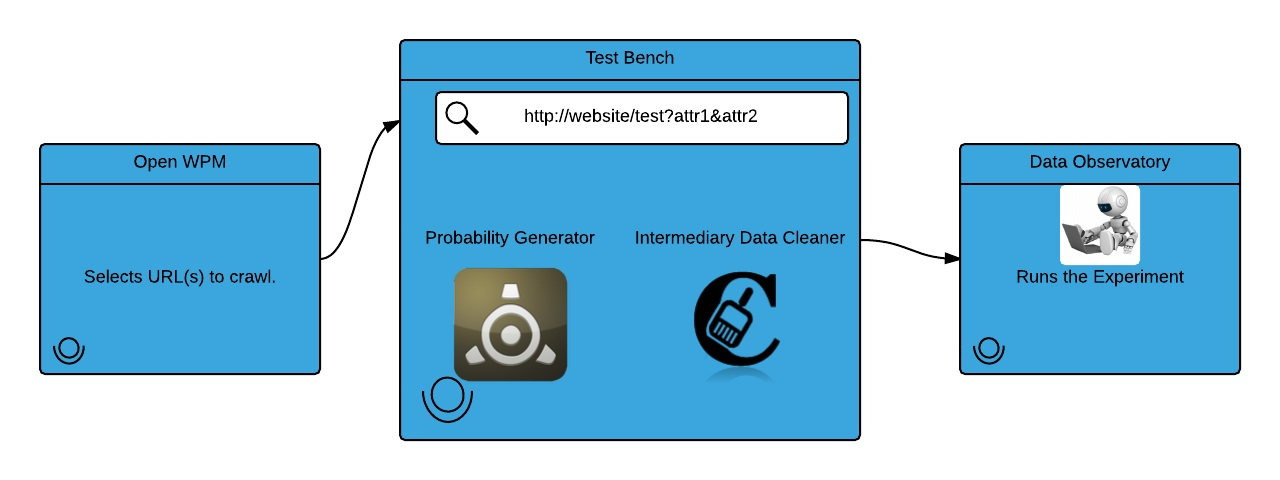
\includegraphics[width=\linewidth]{architecture.jpg}
    \caption{System Architecture}
    \label{fig:architecture}
\end{figure}
\subsection{Overview}
As is evident from the Figure ~\ref{fig:architecture}, OpenWPM supplies the URLS to the Test Bench. Test Bench supports the URL in form of standard URL encoded query parameters. A typical example of query being supplied to Test Bench would be 
\begin{center}
\url{www.testbench.com/test/?gender=male&country=germany}
\end{center}
There is no limit on the number of parameters the system can take. The probability generator interfaces with the configuration file (see configuration in this section) for the desired experiment and renders the DOM for OpenWPM. These web-pages are then stored and asynchronously picked up by Data Observatory for detection.
\subsection{Wrappers}
Our wrappers are connectors which act as bridge between OpenWPM--Test Bench--Data Observatory. They are required because OpenWPM and Data Observatory don’t inherently support interface access. Also since the experiments can be configured from the website, for quality of experiment (see quality in this section), we keep the data separately across the iterations and across the experiments.The wrappers provide a way to set the iterations/number of browsers in an experiment and supply different probability across experiments.
\subsection{Data Observatory Dictionary Generator}
Data Observatory needs some reference of location. So the OpenWPM wrapper modifies the name of the file and appends it with the query-parameter and after its done collecting the data from the website it iterates over the directory which has the generated results and generates mappings to location for each file.  Below is a part of JSON format that we create for the mappings. This JSON has a key \quotes {all\_keys} in which all the geographical locations can be specified.Also one should keep in mind that if this file is not supplied to Data Observatory it will not work correctly. This is not exactly innovation or any contribution from our side, but we are including this for completeness of the report.  
\begin{lstlisting}[language=json,firstnumber=1]
{
	"7_9_localhostcountry=india&
    gender=female.html": {
		"geo": "india"
	},
	"all_values": {
		"geo": [
			"germany",
			"india"
		]
	}
}
\end{lstlisting}
\subsection{Configuration}
Our configuration file is a JSON key-value dictionary shown below. This file is customized per experiment and is kept constant throughout the experiment. New keys and their corresponding values can be easily added and the dictionary can be extended to support many other attributes.
\begin{lstlisting}[language=json,firstnumber=1]
   {
        "country":{
            "germany":{
                "0.1":"German",
                "0.9":"Default"
                },
            "india":{
                "0.5":"Indian",
                "0.5":"Default"
                }
            },
        "gender":{
            "male":{
                "0.7":"Male",
                "0.3":"Static"
                },
            "female":{
                "0.8":"Female",
                "0.2":"Static"
                }
            }

        }
       
\end{lstlisting}
\textbf{Config Structure}
The top level elements specify the keys which are the same in the query-params,the second level correspond to the value of the attribute. We maintain a running counter which generates a random number N(0,1) and updates the counter. This is to ensure the probabilities depend on previous interactions with the system.(see Self-Evaluation for a discussion on probability generations)
\subsection{Data Observatory Wrapper}
The Test bench wrapper interacts with the Data Observatory and does the following:-
\begin{itemize}
\item Extracts only the elements which have corrected P-values.(See Appendix for code snippet)
\item Cleans the Data Observatory intermediate files.(See Quality in next subsection for why its important) 
\item Extracts the P-values and stores it element wise.
\item Stores the results (success/failure) iteration wise for each experiment.
\end{itemize}
\subsection{Quality}
To ensure each iteration has no bias taken from previous interactions, the Test Bench – Data Observatory deletes all the intermediary values. The Data Observatory uses the generated values as a cache for experiments. This is a small bug in the implementation system which can severely skew the P-values. This makes the Data Observatory consider the previous experiment/iteration P-values and sometimes leads to erroneous detection.\par
Apart from that we introduce our own name space format in Data Observatory for storing the result of the experiments. Again we are introducing this only for completeness and to make sure tests are conducted in a clean environment.

\section{Methodology}
With all the basic components in place we can now introduce how we actually conduct the experiments. This section first discusses about the self-evaluation of generated probabilities and iterations. And then discusses about the method we used for for elements testing. The scope of our tests was limited to varying at maximum 2 elements in a DOM independently.

\subsection{Self-Evaluation}
Our goal was to find the minimum number of iterations we must run so that the probabilities that are being generated are stable. This is important because if we cannot guarantee from Test Bench side that the probabilities generated would be constant and reproducible we cannot guarantee whether they would be detected from Data Observatory side.\par
So we decoupled our probability generator and then ran it under decoupled conditions for 10.\par
More discussion on the minimum iterations required is discussed in Section Result.(see Appendix for probability generator code snippet)

\subsection{Single Element Variation}
All the content in the website was fixed and only one attribute (country) was varied.
\begin{table}[h!]
	\begin{center}
    \begin{tabular}{| l | l |}
    \hline
    Probability & Iterations(Maximum) \\ \hline
    0.9 & 288\\ \hline
    0.8 & 242\\ \hline
    0.7 & 288\\ \hline
    0.6 & 288\\ \hline
    0.5 & 288\\ \hline
    0.4 & 450\\ \hline
    0.1 & 800\\ 
    \hline
    \end{tabular}
    \caption{Maximum Running Iterations for Probabilities}
	\label{table:name}
    \end{center}
\end{table}\par
Iterations: In OpenWPM the crawling can be done wither sequentially or using multiple browsers. Each iteration can be then defined as a tuple of (browsers, iterations), hence we defined our iterations as (15, 15) or (12, 12) and so on. Since we were using two URLS for correlations hence the P-values are generated over all the iterations hence (12, 12) becomes 144*2=288 iterations.   In hindsight we could have defined it to some whole number but from an experimental point of view it hardly makes any difference. \par
Secondly the number of iterations might seem different for some of the probability. It’s because once the Data Observatory converges (achieves 100\% detection for a single element), we stop the iteration.\\
OpenWPM crashes after 40*40 browsers and iterations hence that’s the maximum number of iterations we ran for probability of 0.1. More discussion is included in Section Result.

\subsection{Two Elements Variation}
In this experiment we varied two attribute and changed the probability. In some experiments, the probability was kept equal between elements while in some cases we varied them independently (here independence implies probability of one element was not equal to other attribute).



\section{Web System Implementation}
\subsection{Overview}
We used Django as the web application framework for our project. Django is an open source web application framework, written in Python. The main reason that we chose Django as the web application framework is because both OpenWPM and Data Observatory are written in Python. So using a Python web application framework helps make the whole integrated system to be unified and easy to manage.\par
On the side of front end, we used JQuery library and Bootstrap to build the system web pages.\par
Every time when a user wants to display the chart of experiment result, the front end system sends an AJAX call to the back end system to get JSON formatted chat information, and shows that on the web pages.\par
The architecture of the web application is shown in the Figure~\ref{fig:webAppArchiecture}:\par
\begin{figure}[h!]
	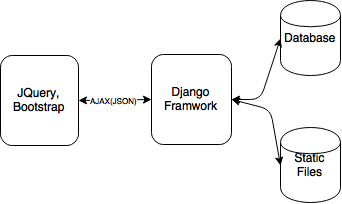
\includegraphics[width=\linewidth]{web_application_architecture.png}
    \caption{Web Application Architecture}
    \label{fig:webAppArchiecture}
\end{figure}
In our test bench application, we created several pages to show various testing settings. From the screen shot of the web system below, we can see the option of “Dry Run Test”, “Single Element Page”, “Multiple Elements Page”, “Test Page”, “Configure Page” and “Visualization”. We will introduce the function of these options in the following sections.

\subsection{Dry Run Test}
\begin{figure}[h!]
	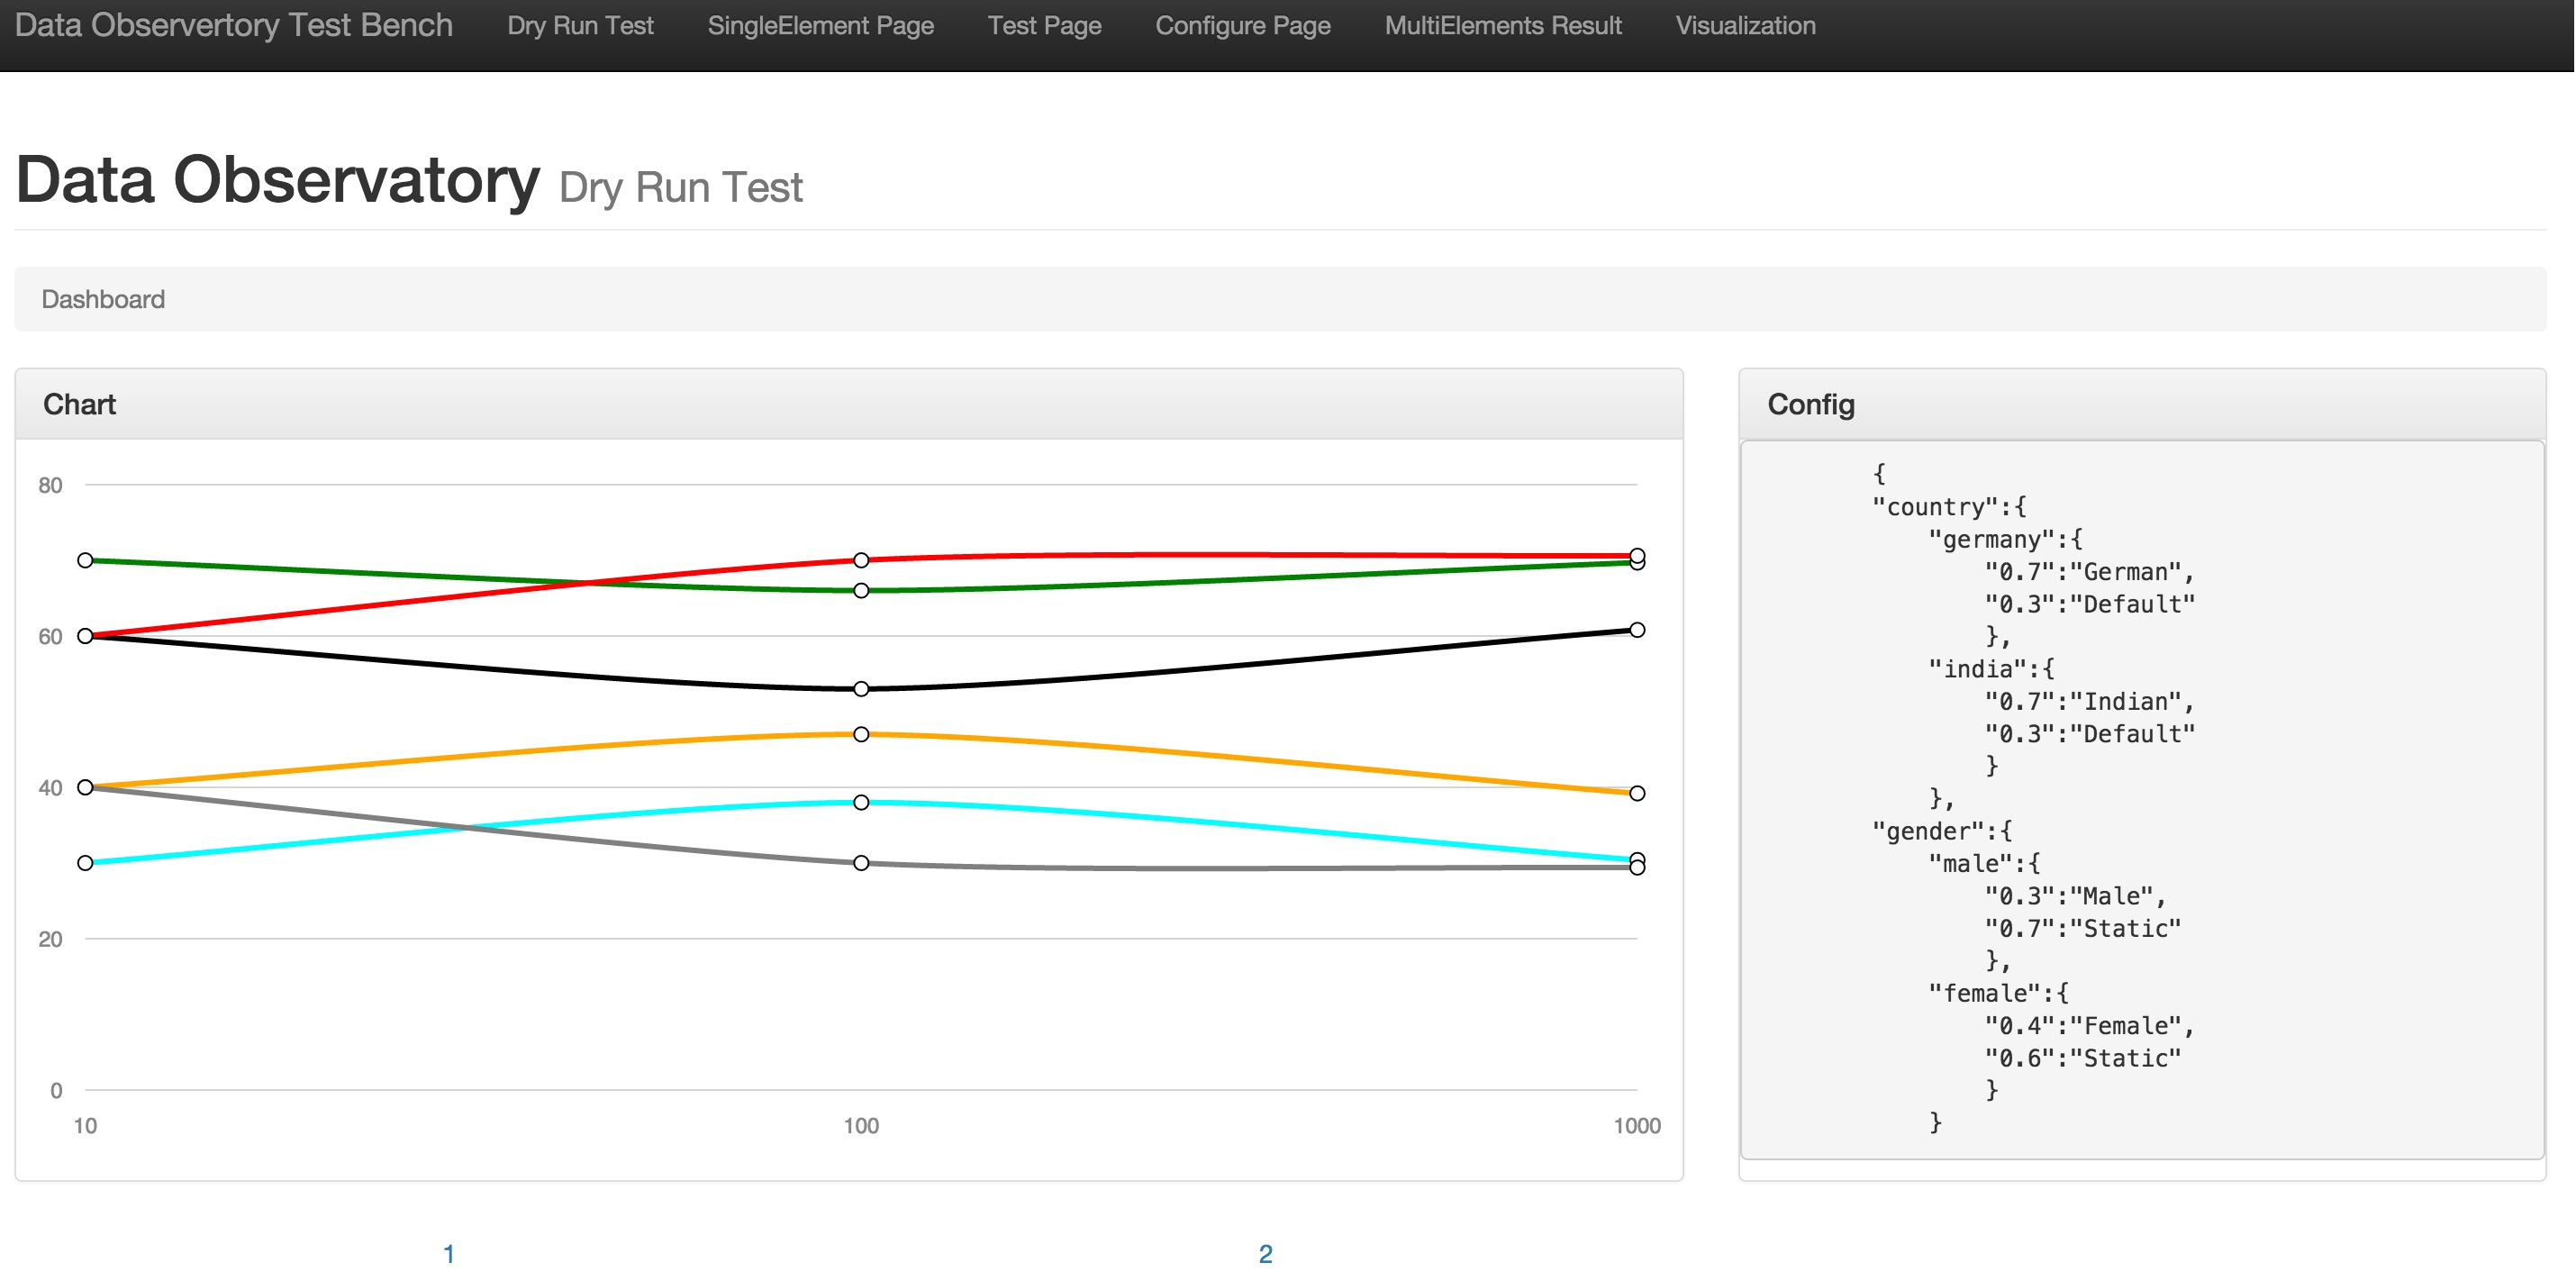
\includegraphics[width=\linewidth]{dryruntest.jpg}
    \caption{Dry Run Test Page}
    \label{fig:dryrun}
\end{figure}
In the Figure~\ref{fig:dryrun}, we display the appearance probability of each element in DOM. If the line is relatively horizontal and becomes stable when the running times becomes long, it means we succeed in generating the DOM elements with the configuration file formatted in JSON. The web page also shows the corresponding testing result of this experiment result on the right side. All data is retrieved from the back end server. We keep the test result in folders named in their IDs of experiments.

\subsection{Single/Multiple Elements Test}
\begin{figure}[h!]
	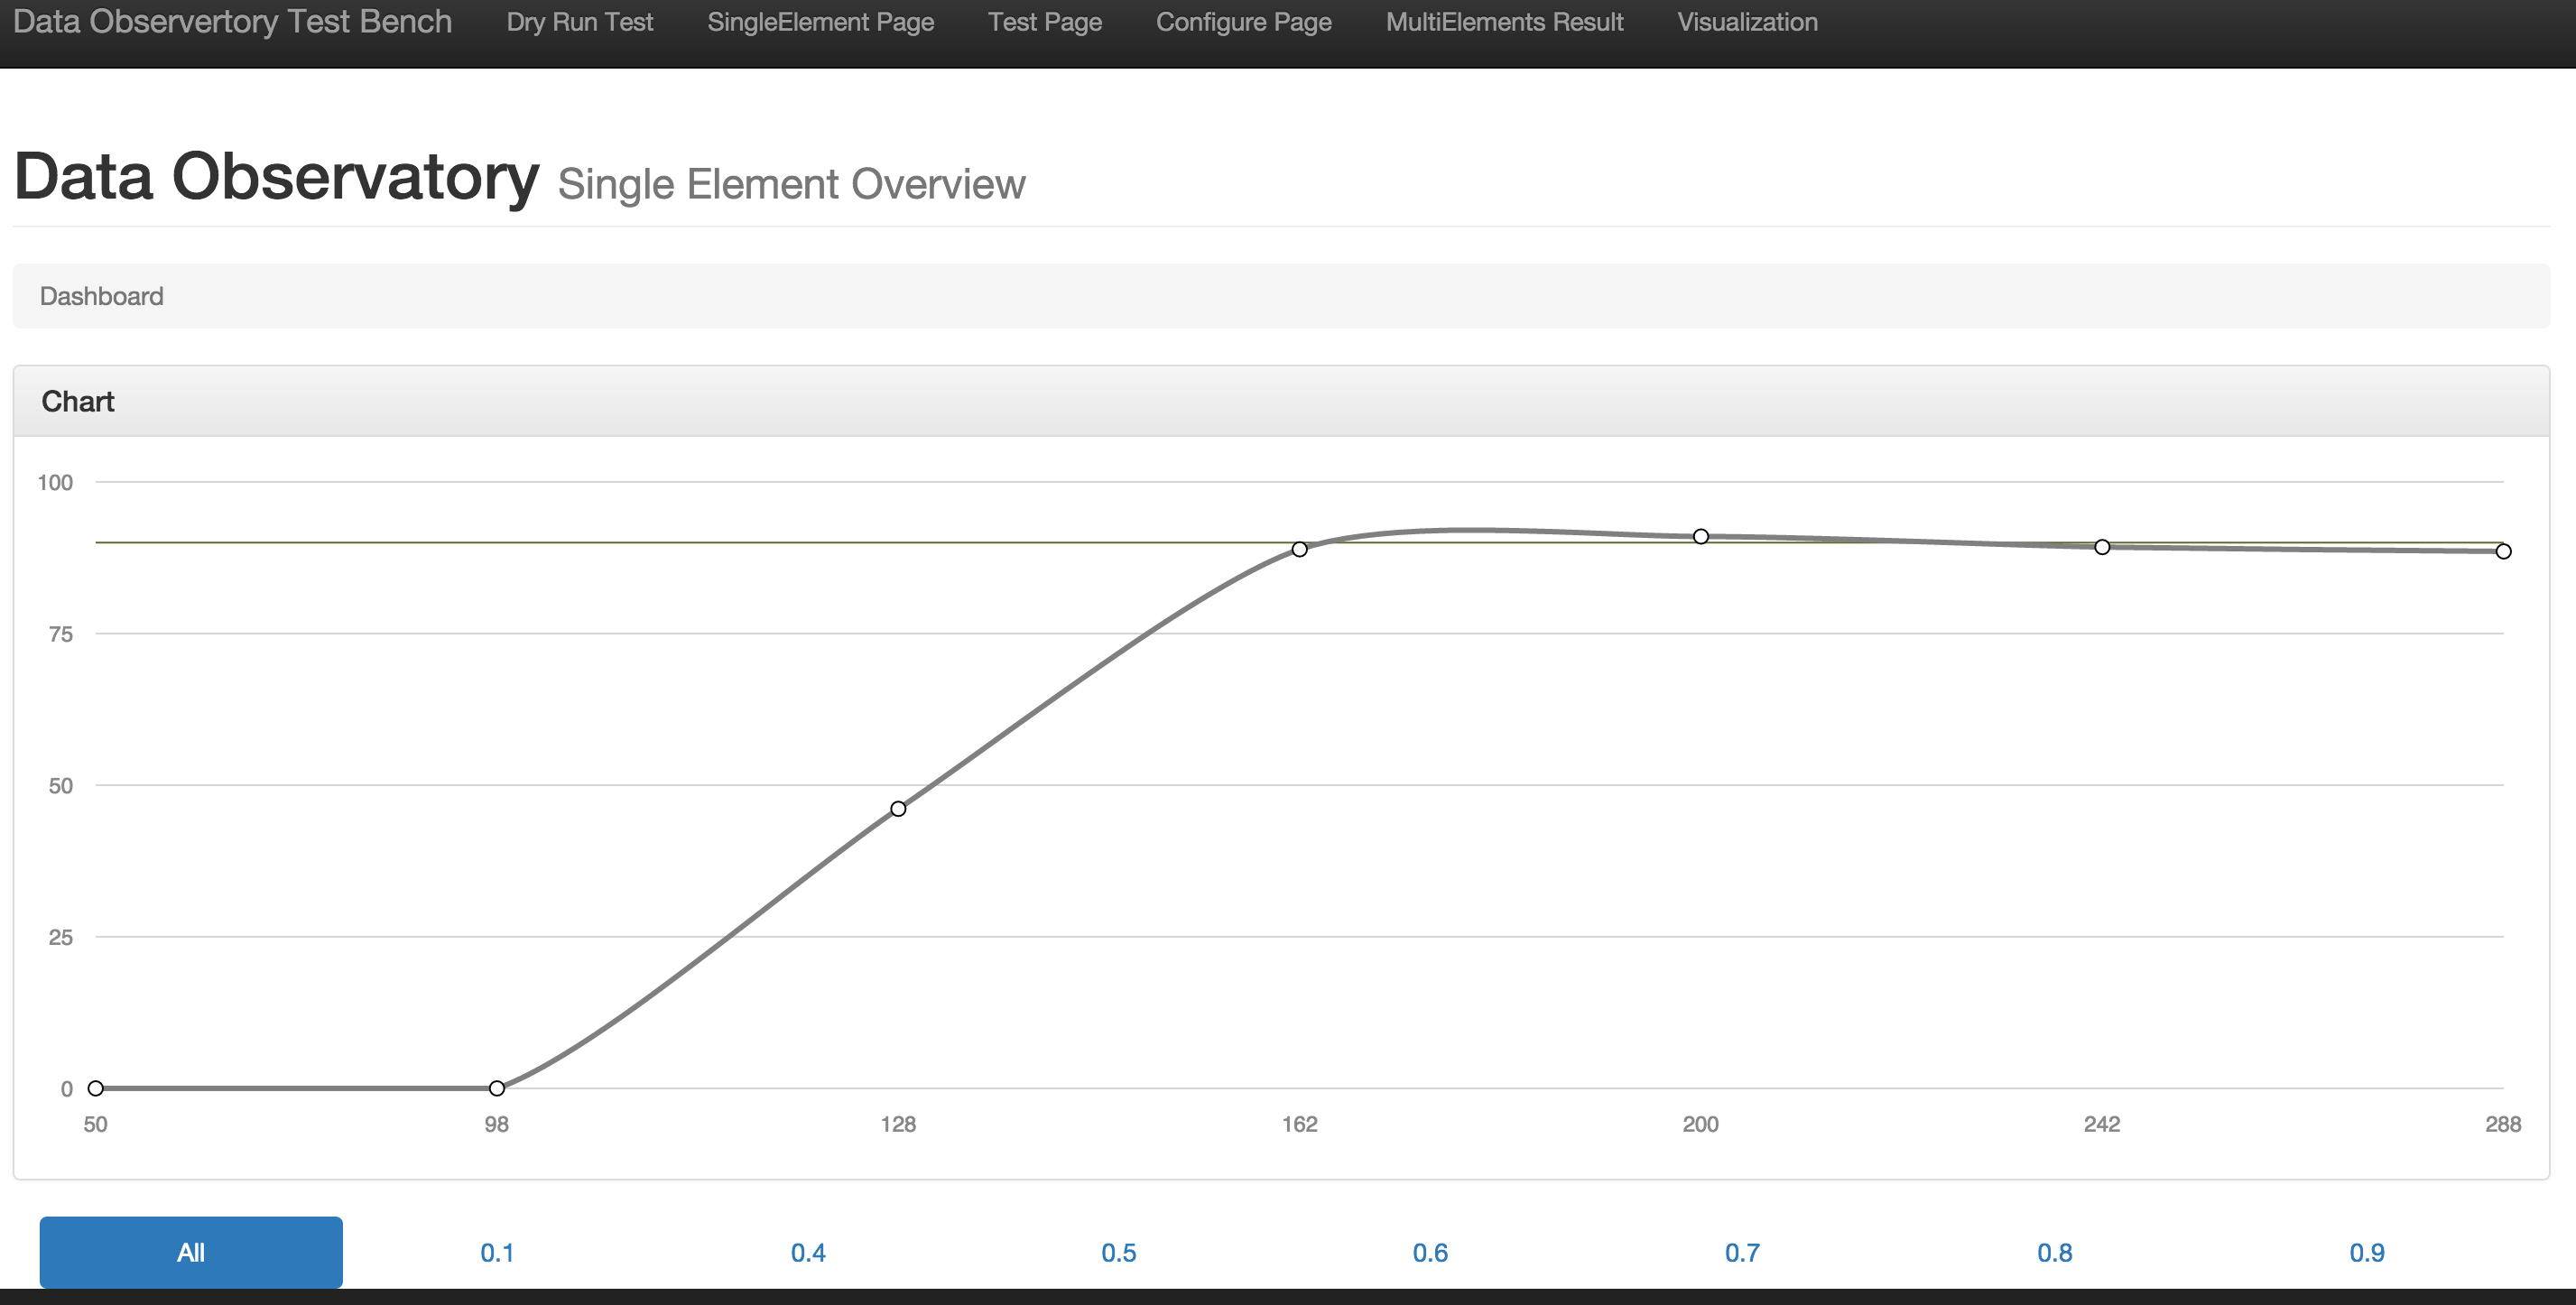
\includegraphics[width=\linewidth]{singleelement.jpg}
    \caption{Single Element Test}
    \label{fig:singleElementTest}
\end{figure}
In both single and multiple elements test pages, we use Morris chart to show the detected success rate. The lighter horizontal straight line is used to show the target success rate and the x axis represents the number of iterations we ran the experiment. The experiment result data is saved in the back-end database with their corresponding probabilities.


\subsection{Test Page}
\begin{figure}[h!]
	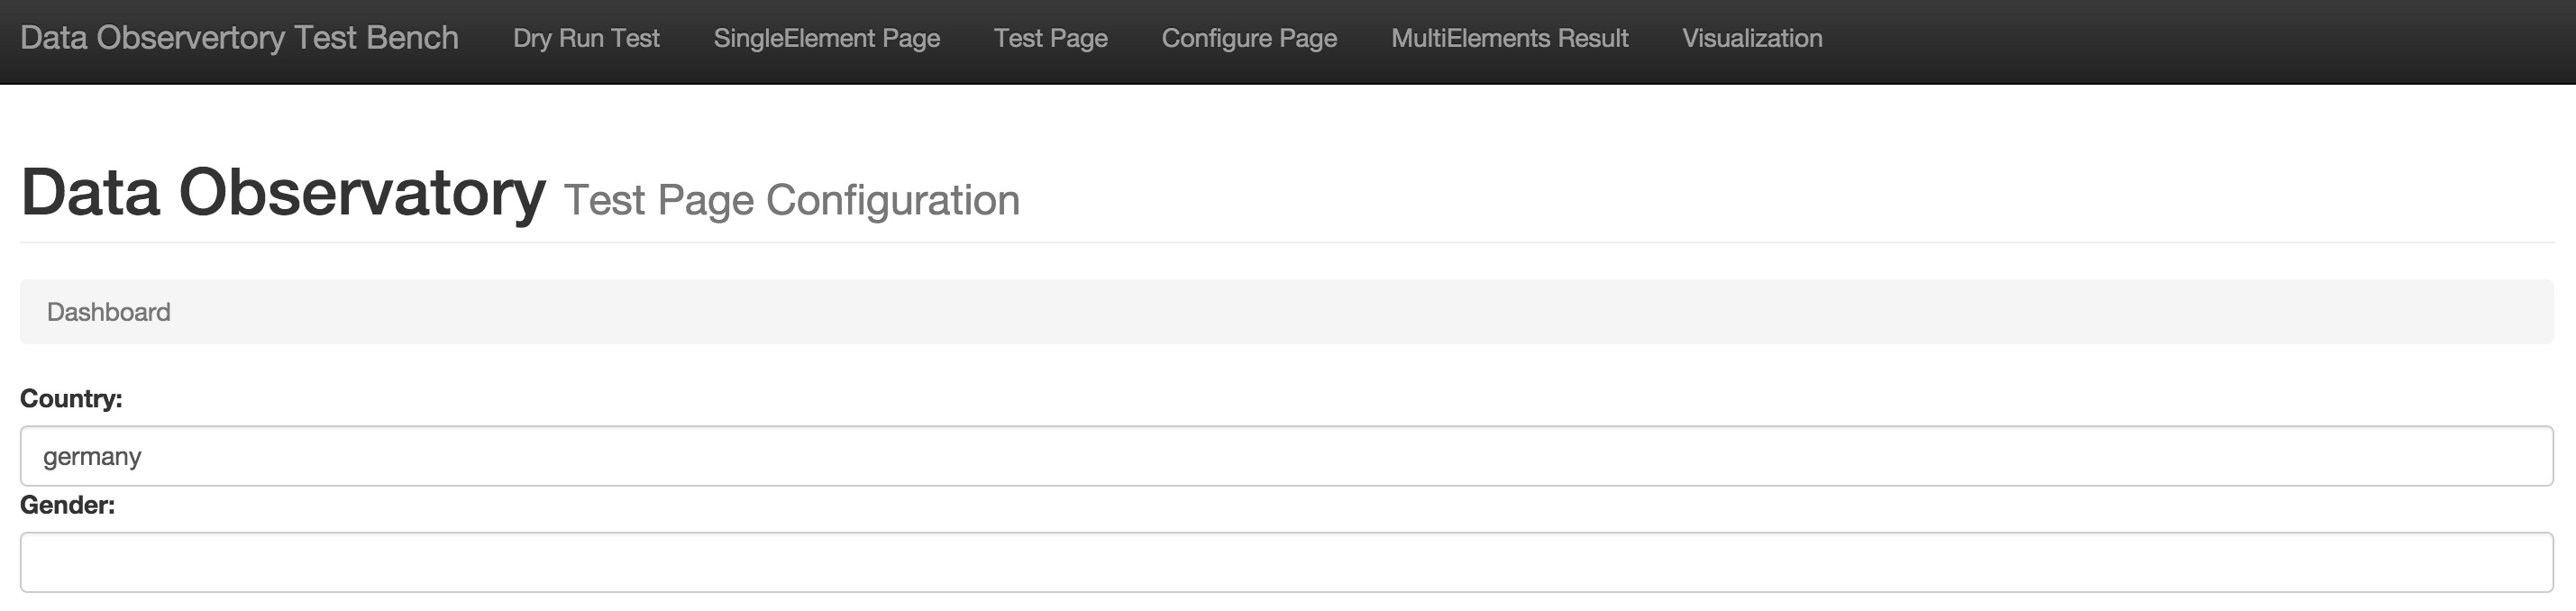
\includegraphics[width=\linewidth]{testpage1.jpg}
    \caption{Test Page Generation Configuration}
    \label{fig:testpage1}
\end{figure}
In the Figure~\ref{fig:testpage1}, the web application requires a user to enter the current country and other information, which will be embedded in the query parameters of test URL. We basically copy the information from the table form and construct a corresponding query URL to ask for a dynamic generated web page.\par
\begin{figure}[h!]
	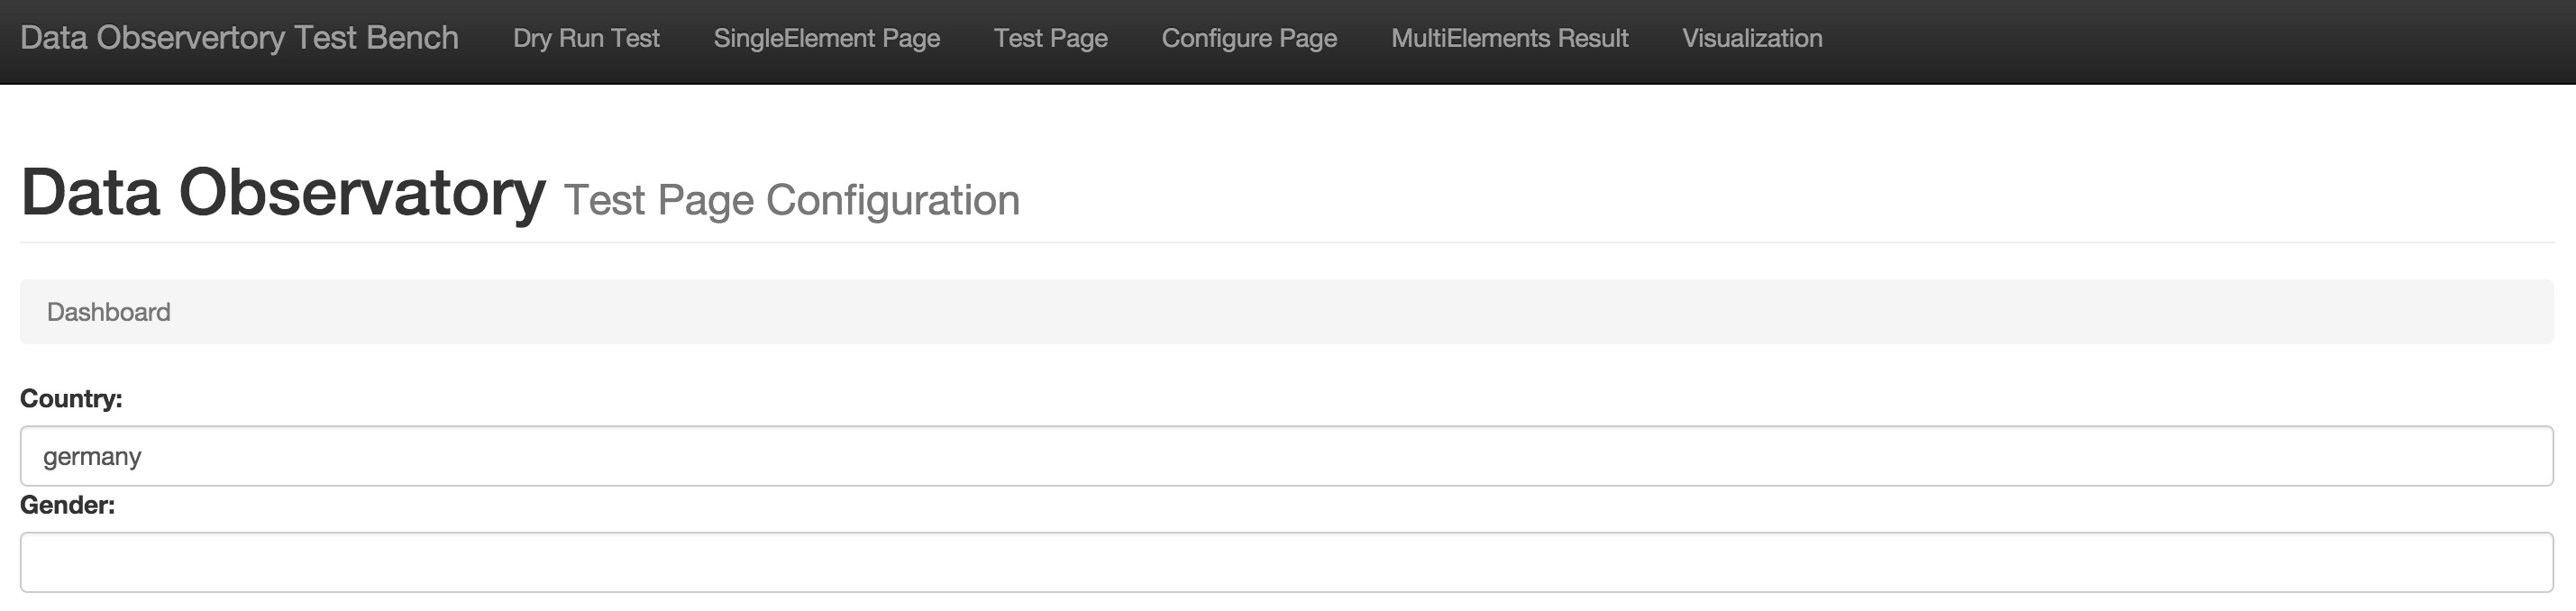
\includegraphics[width=\linewidth]{testpage1.jpg}
    \caption{Test Page}
    \label{fig:testpage2}
\end{figure}
At the back-end system, we made a template in Django to generate the dynamic web-page. The template fills the pattern with elements according to the setting in configuration JSON file. We put some static files (text, photos) in the static fold of Django so that the system can fill them in the place of pattern.

\subsection{Configuration Page}
\begin{figure}[h!]
	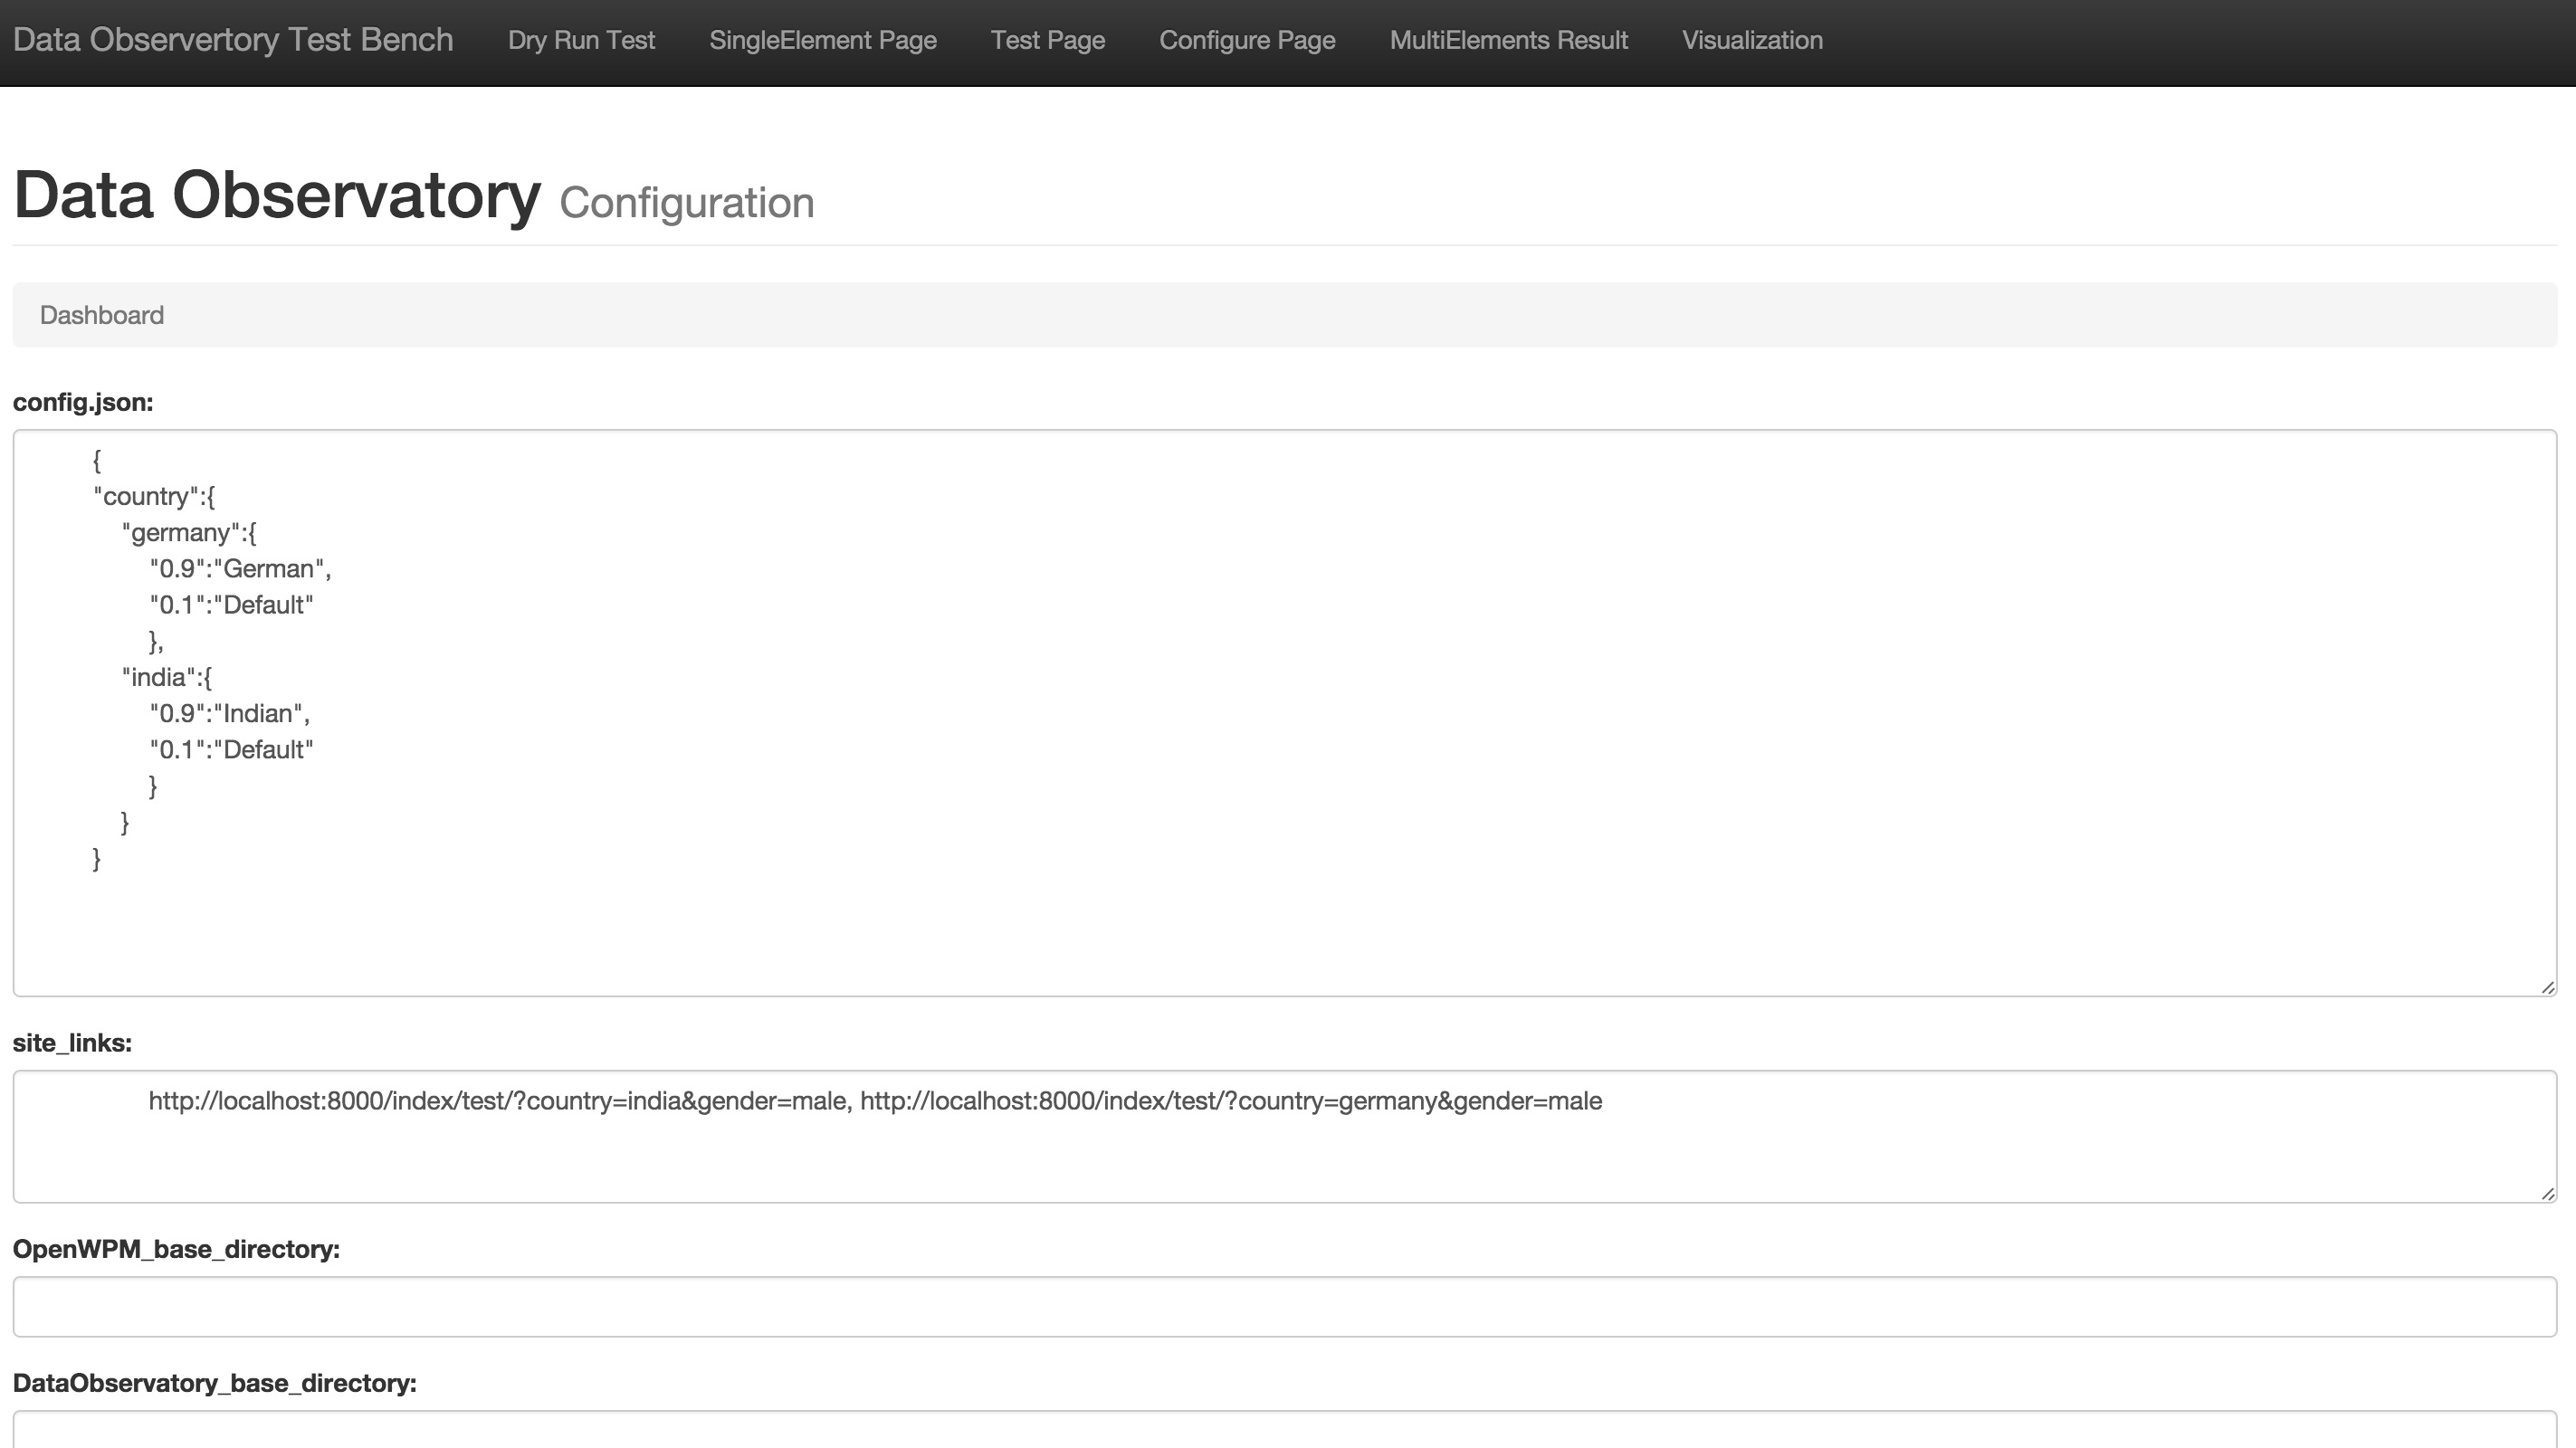
\includegraphics[width=\linewidth]{configurationpage.jpg}
    \caption{Test Bench Configuration Page}
    \label{fig:configuration}
\end{figure}
On the configuration page (Figure~\ref{fig:configuration}), user can change the current probability configuration JSON. Since our script used to run experiment needs to specify the directory of OpenWPM and Data Observatory, we can give the path to these directories on this page. We can also specify the experiment running iterations and output result file names on this page. 

\subsection{Visualization}
\begin{figure}[h!]
	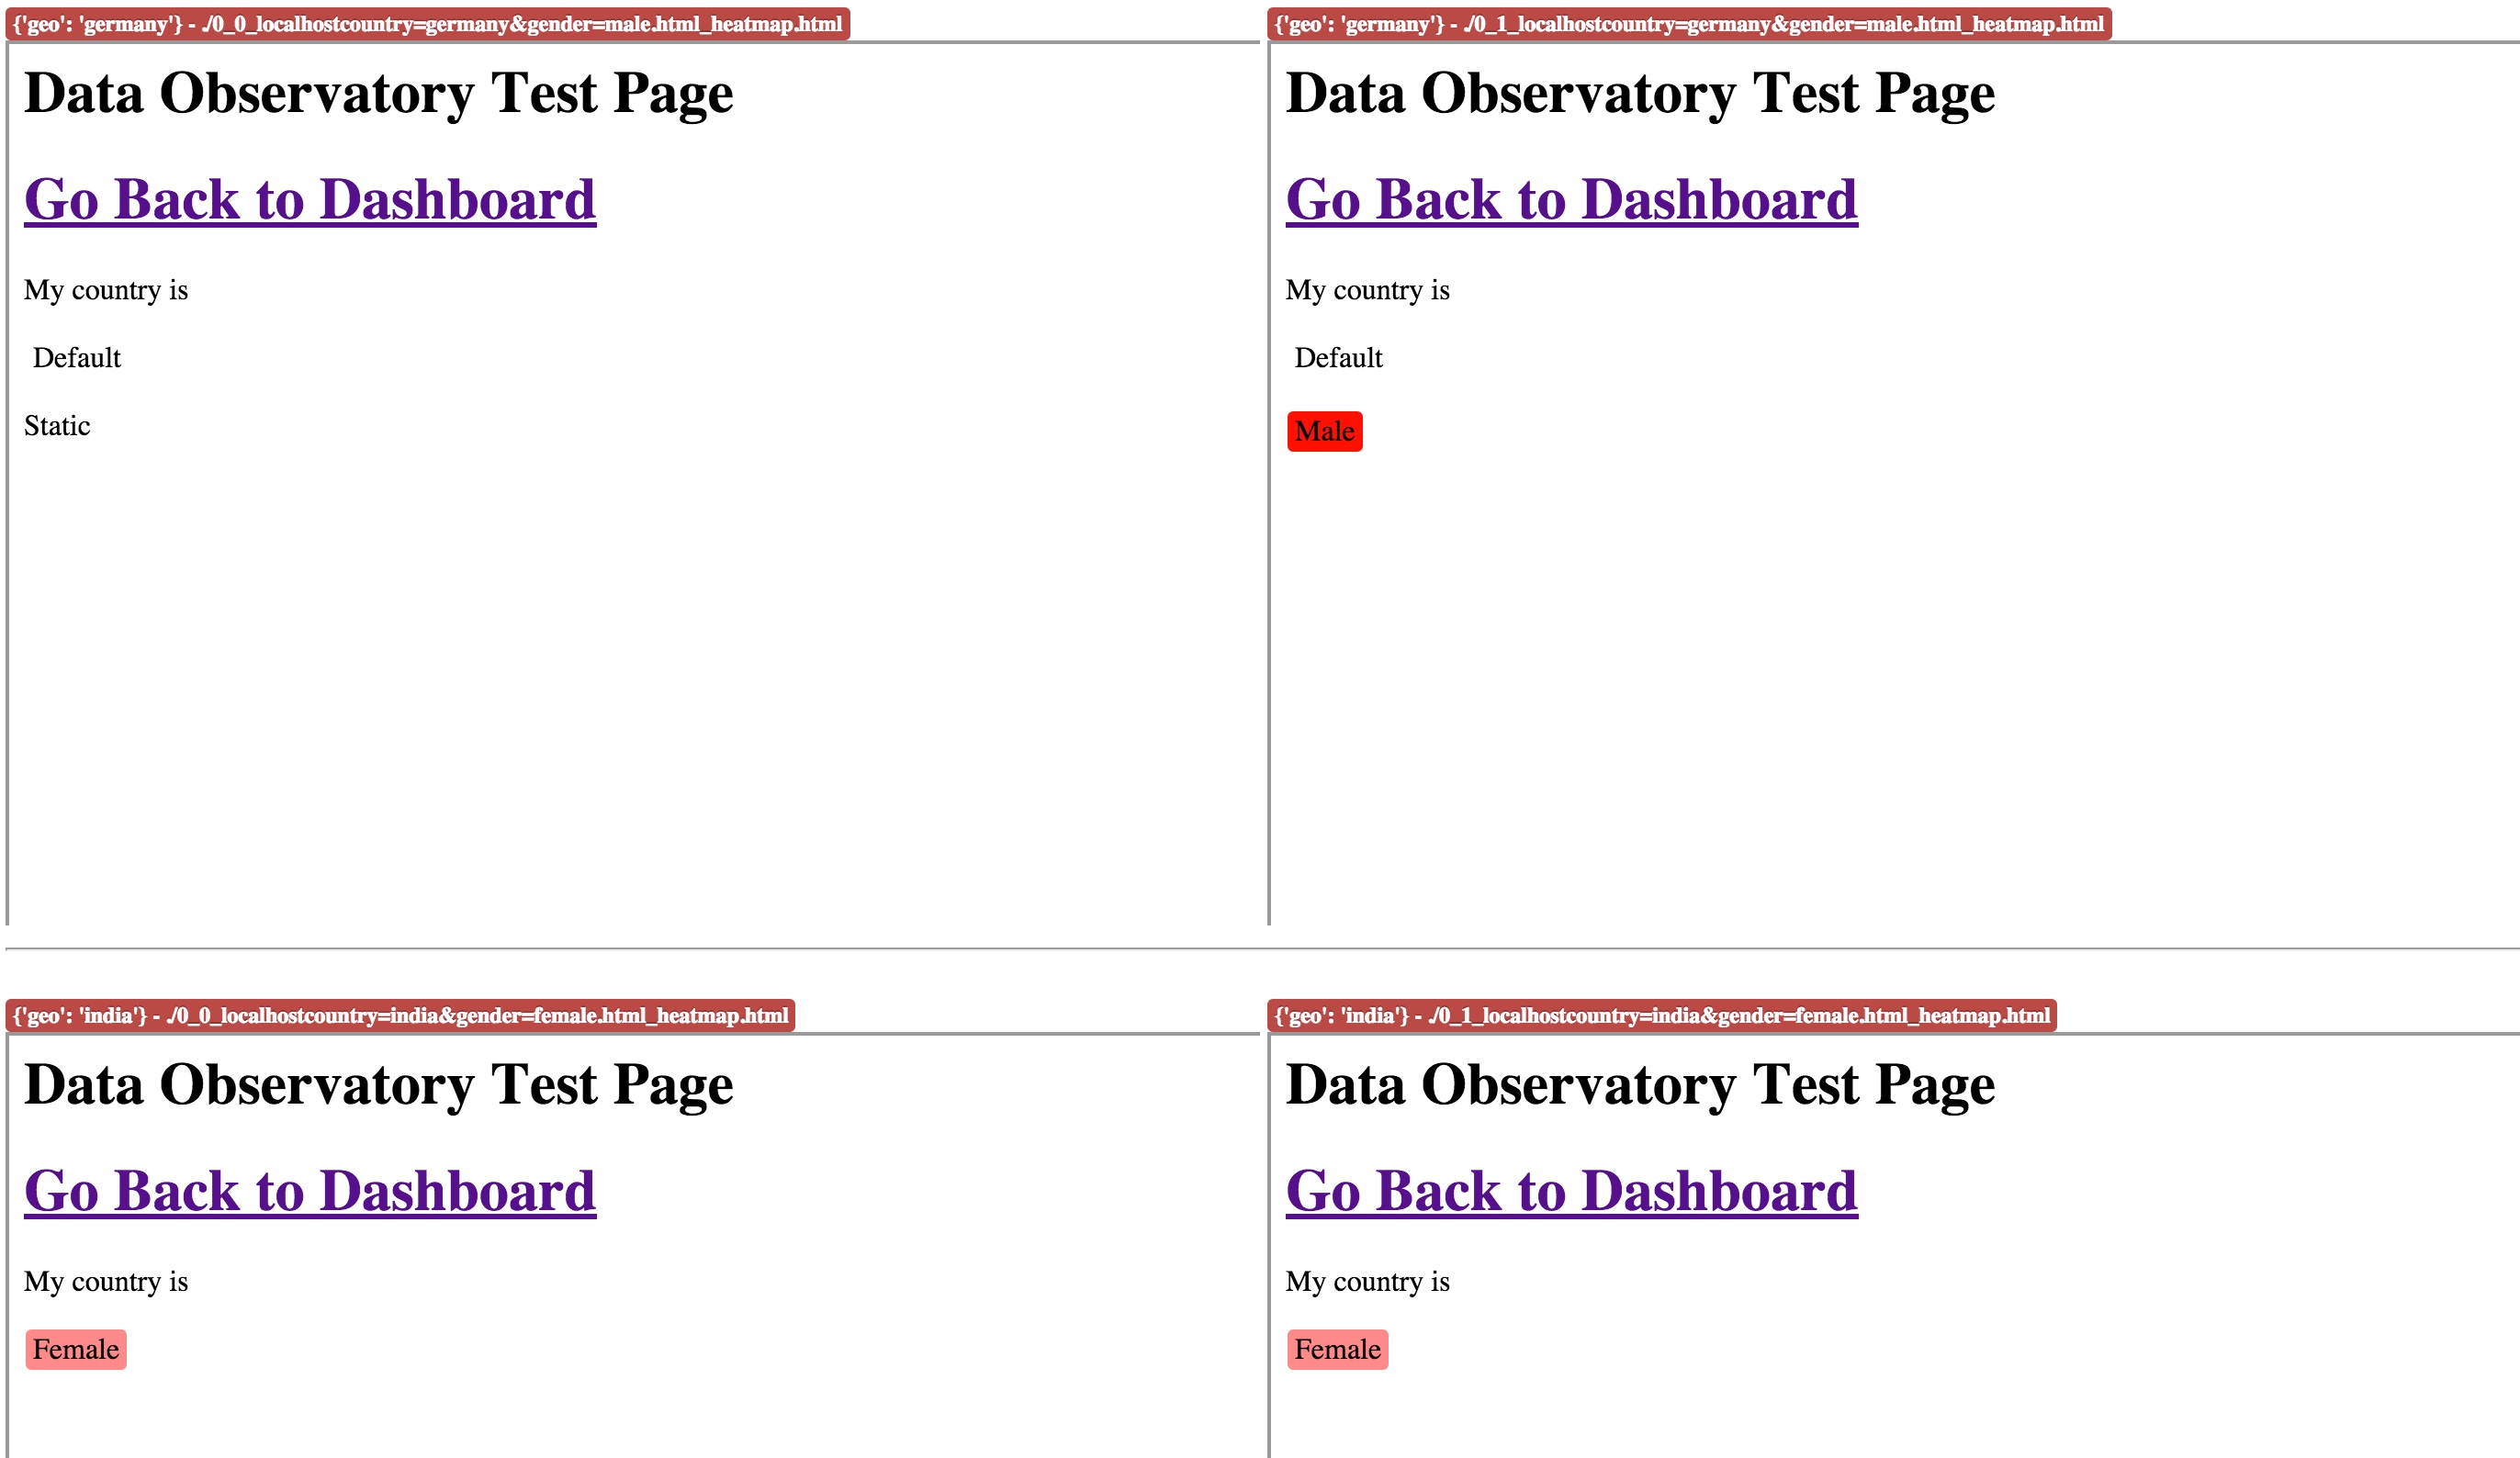
\includegraphics[width=\linewidth]{visualization.jpg}
    \caption{Visualization Page}
    \label{fig:visualization}
\end{figure}
The visualization page is used to show the result web page with annotations. This visualization web page was implemented by the teaching assistant of the course, Yannis Spiliopoulos. And we embed the visualization part into our system for the convenience of displaying experiment results.

\section{Result} \label{result}
While using the above discussed methodology we got the following results.
\subsection{Self-Evaluation}
We ran the self-evaluation for a number of iterations and found that the results on an average converge around 10 $\sim$ 25 iterations hence the minimum number of iterations we should run for Data Observatory should be 25. Since we had six varying elements (‘Default’, German’, ’Indian’, ’Static’, ’Female’, ’Male’) we ran the tests in one go for all the elements and counted the number of times Test Bench generated the element.  Y axis specifies percent of time the element was generated and  X axis denotes the number of iterations we ran for that particular element.Finally Figure ~\ref{fig:Evaluation Results of Probability Generator} looks consistent with our expectations.Each title of a subplot shows the name and probability of element.
\begin{figure*}[h!]
	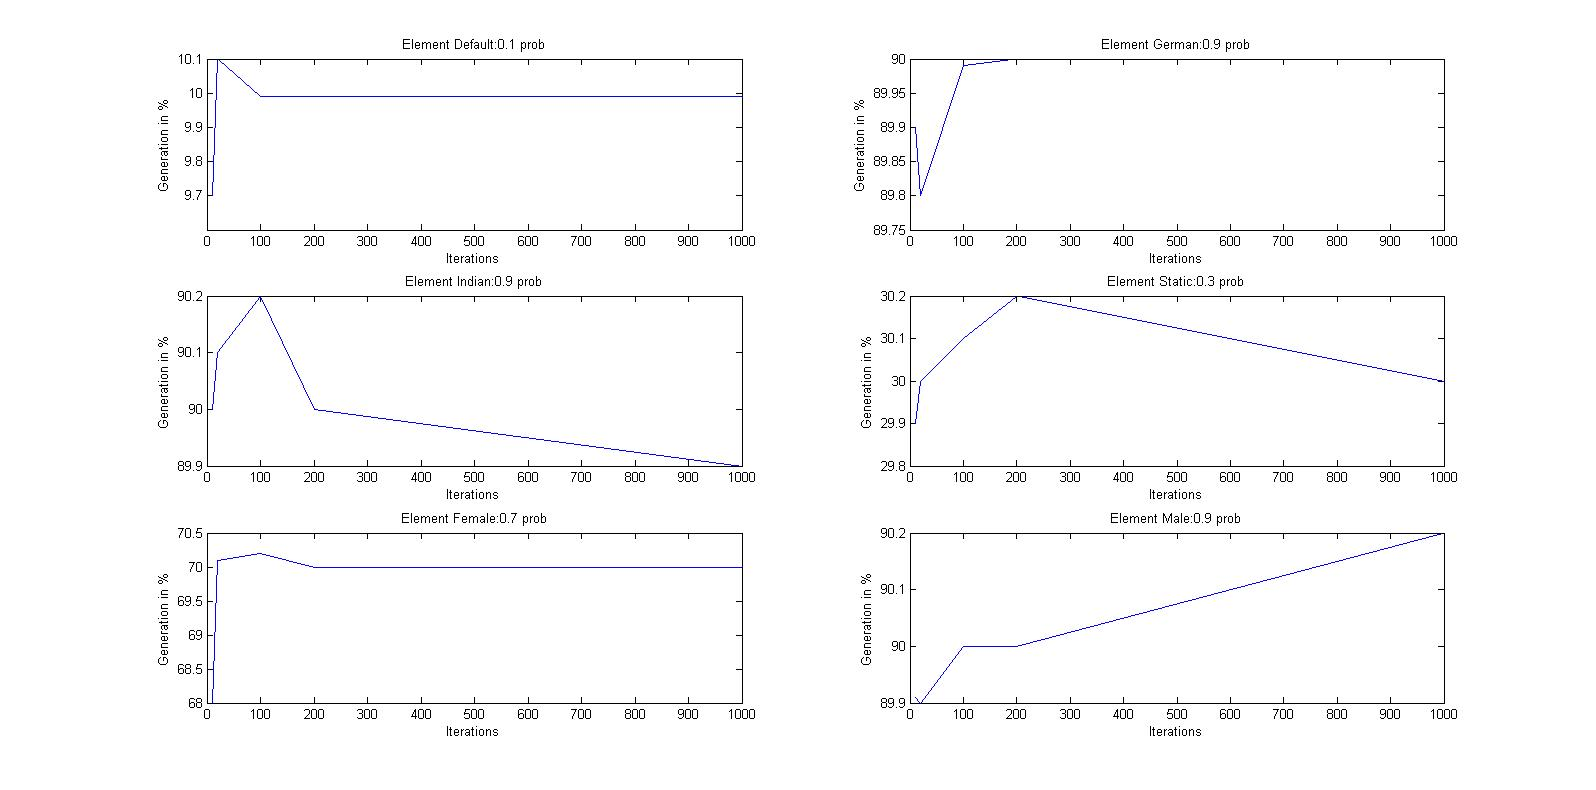
\includegraphics[width=\linewidth]{self_evaluation_results.jpg}
    \caption{Self Evaluation}
    \label{fig:Evaluation Results of Probability Generator}
\end{figure*}

\subsection{Single Element}
For single element per Experiment we ran sets of iterations and calculated the number of elements having P-values less than the threshold. \par
Table ~\ref{table:iterations} gives an idea of the number of iterations we ran for each experiment. \par
In Figure ~\ref{fig:singleElementResult},Y axis denotes the percentage of elements which had P-values which had less than the threshold and the Title of each graph denotes the maximum percentage of elements allowed to have that value.Also X axis denotes the number of iterations that we ran for that particular experiment. To illustrate further let’s say we run an experiment with 0.9 then in 100 iterations that element should have P value less than threshold at max 90 times. \par
Furthermore discussing on the results we can see that even in case of high probability (0.9), we must run at-least 200 iterations to be sure that the element can be detected. The detection becomes more difficult at lower probabilities and it reverses at 0.5. As is evident from graph it crosses the maximum detection range of 50 \% and start detecting elements which were not supposed to be detected. Also if the probability of appearance of element is less than 0.4 it fails even after 800 iterations.
\begin{table}[h!]
	\begin{center}
    \begin{tabular}{| l | l |}
    \hline
    Probability & Maximum Iterations \\ \hline
    0.9& 288\\ \hline
    0.8 & 288\\ \hline
    0.7 & 288\\ \hline
    0.6 & 288\\ \hline
    0.5 & 288\\ \hline
    0.4 & 800\\
	\hline
    \end{tabular}
    \caption{Iterations}
	\label{table:iterations}
    \end{center}
\end{table}

\begin{figure*}[h!]
	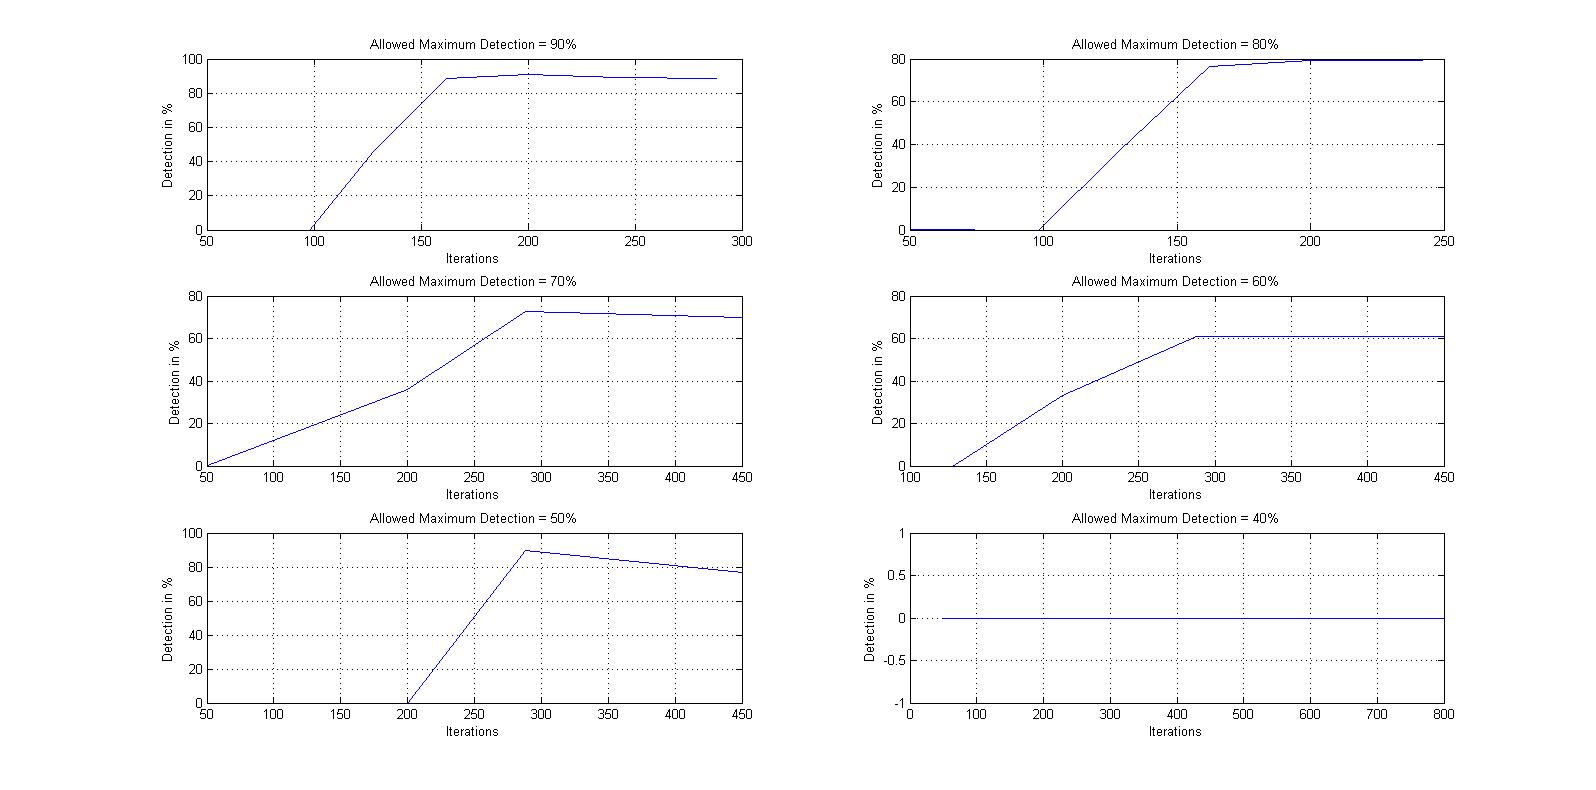
\includegraphics[width=\textwidth]{single_element.jpg}
    \caption{Single Element Result}
    \label{fig:singleElementResult}
\end{figure*}
\subsection{Two Elements}
Interestingly detection becomes more erroneous and tricky when Data Observatory is presented with elements that vary with different individual probabilities. We believe these results require individual attention per experiment so unlike single element, we will be showing each experiment result separately.\par

\textbf{Case 1} Table ~\ref{table:config9} shows the first graph where the elements have the listed probabilities. As we can see from the graph some of the elements which were for the same number of iterations being detected easily have dropped down significantly in their detection percentage. 
\par Table ~\ref{table:config9} shows the detection percentage for each of the element. Interestingly some of the elements (static, default) have not at all been detected although probabilities were low.~\ref{fig:case1results}

\begin{table}[h!]
	\begin{center}
    \begin{tabular}{| l | l |}
    \hline
    Element & Probability \\ \hline
    Indian & 0.9\\ \hline
    German & 0.9\\ \hline
    Female & 0.9\\ \hline
    Male & 0.9\\ \hline
    Default & 0\\ \hline
    Static & 0\\
    \hline
    \end{tabular}
    \caption{Case 1 Configuration}
	\label{table:config9}
    \end{center}
\end{table}
\begin{figure*}[h!]
	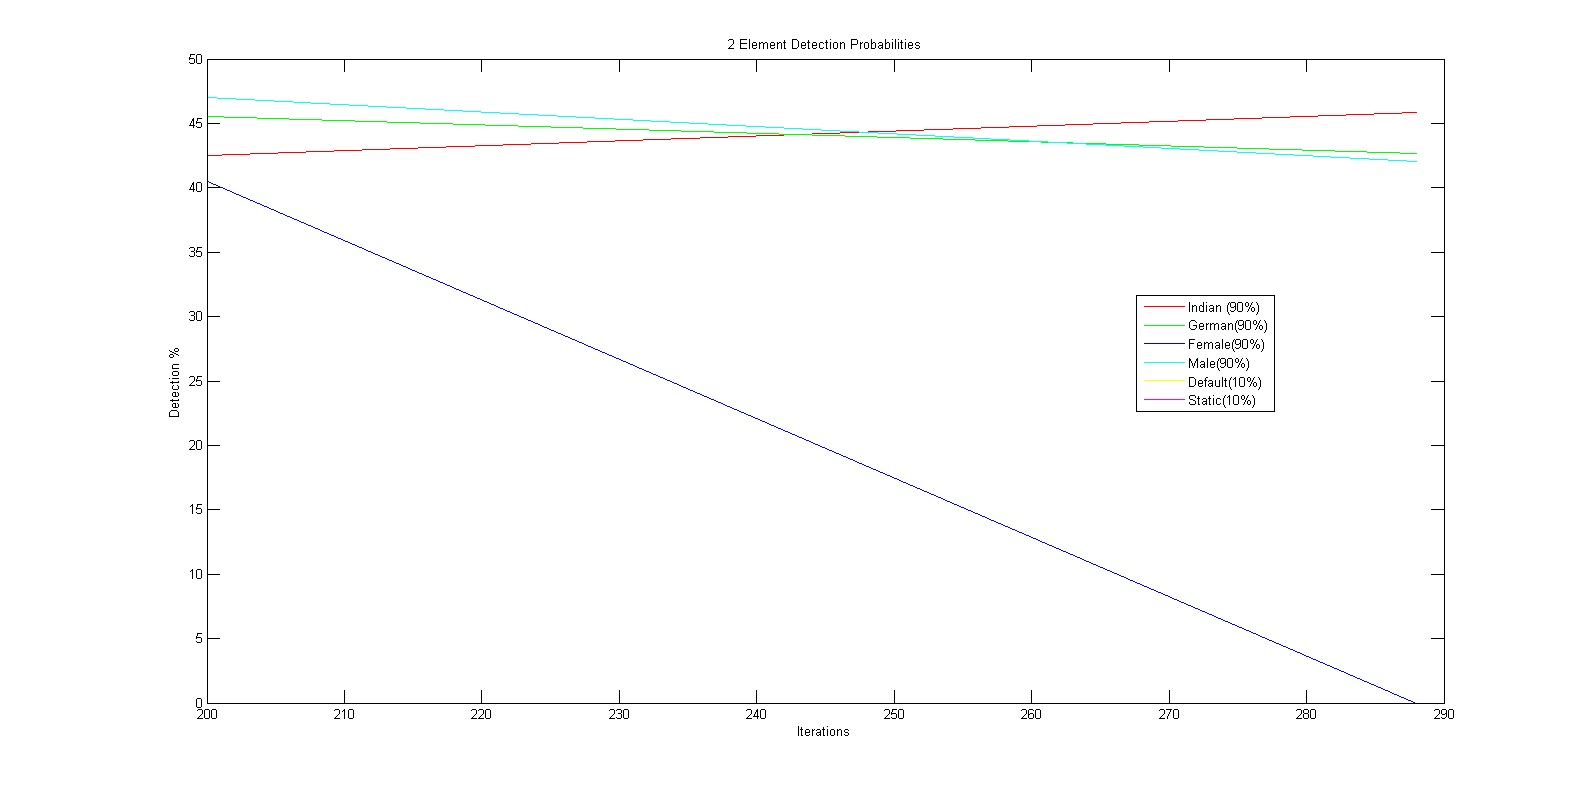
\includegraphics[width=\linewidth]{2_element.jpg}
    \caption{Case 1 Results}
    \label{fig:case1results}
\end{figure*}
\begin{table}[h!]
	\begin{center}
    \begin{tabular}{| l | l | l |}
    \hline
    Element & Iteration 200 & Iteration 288 \\ \hline
    Indian & 42.5 & 42.7\\ \hline
    German & 45.5 & 45.83\\ \hline
    Female & 40.5 & 0\\ \hline
    Male & 47.0 & 42.01\\ \hline
    Default & 0 & 0\\ \hline
    Static & 0 & 0\\
    \hline
    \end{tabular}
    \caption{Results for Case 1}
	\label{table:results}
    \end{center}
\end{table}
 
Obvious anomaly is with Element “Female” which was detected in First iteration but was missing in the second Iteration. Interestingly it did not appear even once whereas other elements like “Male” had a small dip in probability when iteration was increased.
\par \textbf {Case 2} In this case we consider the elements with different probabilities as shown in Table ~\ref{table:case2}. As is evident from the table that few elements have lower and different probabilities from each other. Table ~\ref{table:resultscase2} shows the tabulated results for case 2.
\begin{figure*}[h!]
	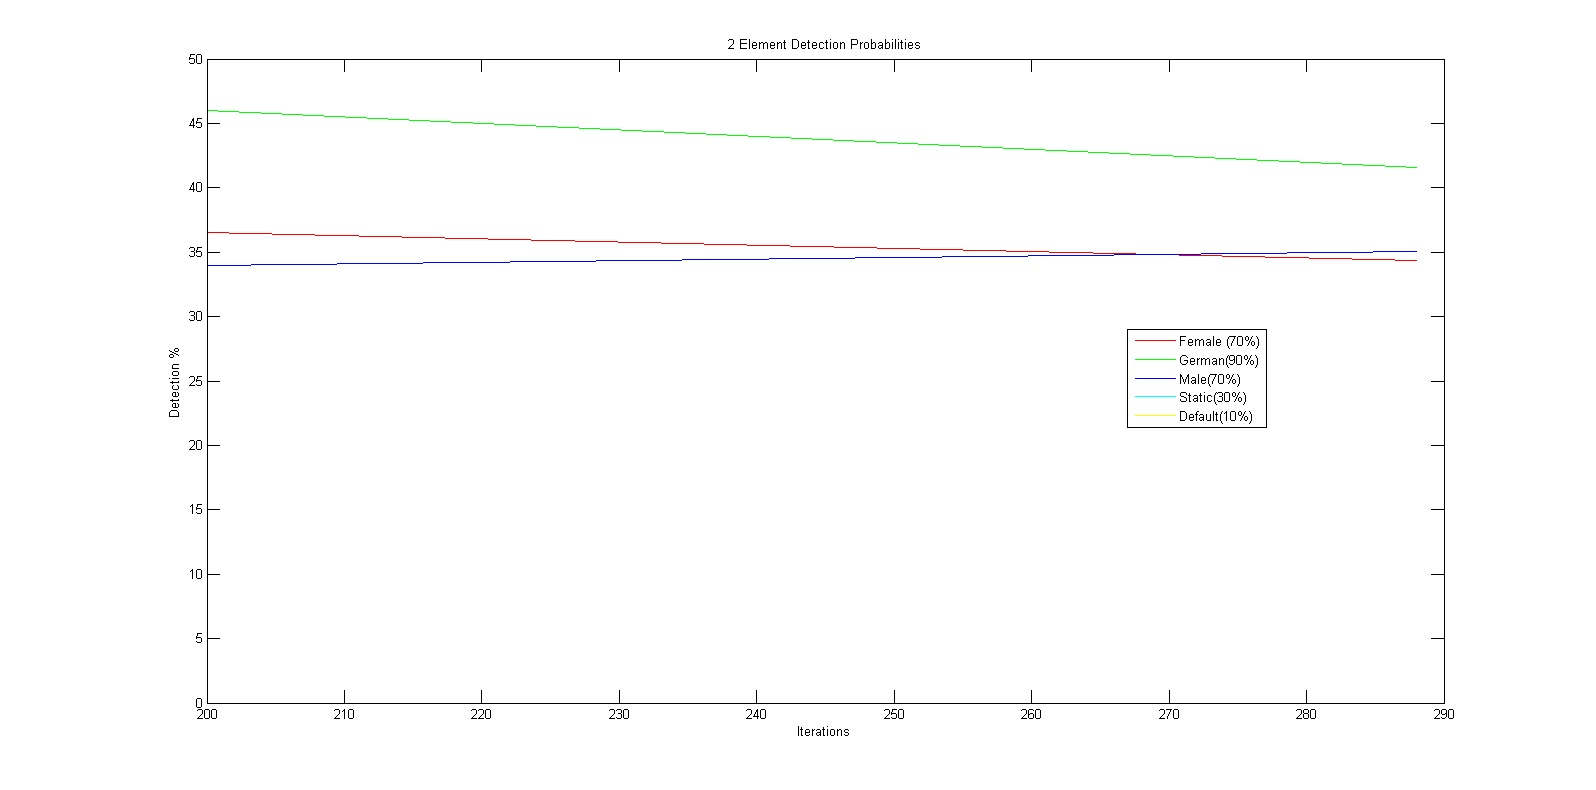
\includegraphics[width=\linewidth]{case2.jpg}
    \caption{Case 2 Results}
    \label{fig:case2results}
\end{figure*}
\begin{table}[h!]
	\begin{center}
    \begin{tabular}{| l | l |}
    \hline
    Element & Probability \\ \hline
    Female & 0.7\\ \hline
    German & 0.9\\ \hline
    Male & 0.7\\ \hline
    Static & 0.3\\ \hline
    Default & 0.1\\ \hline
    \hline
    \end{tabular}
    \caption{Case 2 Configuration}
	\label{table:case2}
    \end{center}
\end{table}

\begin{table}[h!]
	\begin{center}
    \begin{tabular}{| l | l | l |}
    \hline
    Element & Iteration 200 & Iteration 288 \\ \hline
    Female & 36.5 & 34.375\\ \hline
    German & 46 & 41.6\\ \hline
    Male & 34 & 35.06\\ \hline
    Static & 0 & 0\\ \hline
    Default & 0 & 0\\ \hline
    \hline
    \end{tabular}
    \caption{Results Case 2}
	\label{table:resultscase2}
    \end{center}
\end{table}
Figure ~\ref{fig:case2results} shows the detection percentage graph for each element. 
When we vary the element probability differently across attributes we can see that the results are more or less consistent among the iterations. Two elements “Default” and “Static” were not detected in this case. This also does not show degradation in detection performance if the number of iterations are increased.

\section{Conclusions}
\subsection{Single Element}
For single attribute variation we would like to conclude that the system will not be able to differentiate if its probability of appearance is less than 0.4. Also at 0.5 we get abnormal detection. So the element that is appearing frequently in the website should appear more than 50\% on an average to be detected. Also we would like to add that in practical scenarios the content that is shown to users from different locations (taking example of Booking.com) are so different that it would always detect, whereas if elements are varied with less probability detection might not happen.

\subsection{Multiple Elements}
For multiple elements, Data Observatory for the same number of iterations and all other parameters (attribute wise) remaining the same is not able to detect all the elements. We see a drop on average of 50\%. Furthermore we have seen cases in which the Data Observatory stops detecting a particular element, again this can be attributed to the fact that the element’s appearance probability is very low (~0.4). So if a website varies lots of content each with different probability analogy being using more attributes to personalize the content Data Observatory might miss some of the elements. Also contrary to our expectations in some cases increasing the number of iterations reduces the probability of detection. We were not able to find any reason for this behavior even after running multiple iterations on same/under same conditions data set. 


%------------------------------------------------
\phantomsection
\section*{Acknowledgments} % The \section*{} command stops section numbering

\addcontentsline{toc}{section}{Acknowledgments} % Adds this section to the table of contents

We would like to thank the teaching assistant of this course, Yannis Spiliopoulos, for his great help on understanding Data Observatory and OpenWPM, and his advice on system design of this test bench. We would also like to thank Professor Roxana Geambasu for her teaching us the knowledge on the course and advice on designing this test bench system.

\phantomsection
\addcontentsline{toc}{section}{Contributions}
\section*{Contributions} % The \section*{} command stops section numbering
\textbf{Shivam Choudhary}: Designed OpenWPM/Data Observatory Wrapper API; Designed the success-based experiment; Designed Elements-Evaluation testing experiment; Helped in  designing OpenWPM/Data Observatory integration system structure.\\\\
\textbf{Wenyu Zhang}: Implemented Django web application system; Designed test scripts and DOM generation scripts; Designed Self-Evaluation testing experiment; Helped in designing OpenWPM/Data Observatory integration system structure and Wrapper API.

\phantomsection
\section*{Appendix} \label{Appendix}
\addcontentsline{toc}{section}{Appendix}
\ \textbf {Probability generator}
This snippet is the probability generator which takes into account the previous interactions with the system using the SumK variable.
\begin{lstlisting}[language=Python,caption = probability generator]
def make_dom(dict):
    attr_dict = {}
    base_attributes = Common.read_config()
    config = Common.open_config()
    for k,v in dict.iteritems():
        if k in base_attributes:
            p = random.random()
            sumK = 0
            attr_values = config[k][v]
            for k1 , val1 in attr_values.iteritems():
                sumK += float(k1)
                if (p<sumK):
                    attr_dict[k] = val1
                    break
    return attr_dict
\end{lstlisting}

\ \textbf {diff.py code changes}
We modified the diff.py code to extract the elements which have P-values less than 0.001. This snippet extracts those elements and puts them in  a name-space file(code not shown here)\par
\begin{lstlisting}[language=Python,caption = Diff.py changes for generating files]
if correct_pvalues[element_id] is not None:
	pvalf[idx][element] = {}
	for k,v in correct_pvalues[element_id].items():
		pvalf[idx][element]['geo']  =k
		pvalf[idx][element]['pvalues'] = v
		if v < 0.001:
			pvalf[idx][element]['detected']=True
		try:
			counter[element] +=1
		except Exception as e:
			counter[element] = 0

\end{lstlisting}
\ \textbf{File Structure}
Below shows the generated JSON file structure that we use. This shows that along with each element we capture its P-value and calculate the counts as well. File is truncated for brevity.
\begin{lstlisting}[language=json,firstnumber=1]
  {
	"0": {
		" Female": {
			"geo": "geo_india",
			"detected": true,
			"pvalues": 0.00014983087028584553
		}
	},
	"1": {},
	"2": {
		" Male": {
			"geo": "geo_germany",
			"detected": true,
			"pvalues": 0.00010966471321926009
		},
		" Default": {
			"geo": "geo_germany",
			"pvalues": 0.022174198597158863
		}
	},
	"3": {
		" Default": {
			"geo": "geo_germany",
			"pvalues": 0.022174198597158863
		},
		" Female": {
			"geo": "geo_india",
			"detected": true,
			"pvalues": 0.00014983087028584553
		}
	},
	"4": {
		" Male": {
			"geo": "geo_germany",
			"detected": true,
			"pvalues": 0.00010966471321926009
		}
	},
	"detected_counter": {
		" Male": 34.0,
		" Female": 35.5
	}
}
\end{lstlisting}

%----------------------------------------------------------------------------------------
%	REFERENCE LIST
%----------------------------------------------------------------------------------------
\begin{thebibliography}{9}
\bibitem{booking} 
Yannis Spiliopoulos, Differences on prices shown to users from different countries,
\\\texttt{http://www.cs.columbia.edu/\\\~yannis/stable/booking\_com\_us\_ger\\\_LA\_feb01\-feb02\_exp}
 
\bibitem{openwpm} 
Englehardt, S., Eubank, C., Zimmerman, P., Reisman, D., \& Narayanan, A. . 
\textit{OpenWPM: An Automated Platform for Web Privacy Measurement}.
 
\bibitem{domtool} 
Yannis Spiliopoulos,
\\\texttt{https://github.com/columbia/\\data-observatory/blob/master/\\dom\_tools/diff.py}
\bibitem{testbench} 
Shivam, Wenyu
\\\texttt{https://github.com/shivamchoudhary\\/e6998}
\end{thebibliography}
%----------------------------------------------------------------------------------------

\end{document}